\chapter{Empirical Results}\label{chap:mainresults}
\todo{chapter intro} The approach usually starts with the problem definition and continues with what you have done. Try to give an intuition first and describe everything with words and then be more formal like `Let $g$ be ...'.

Start with a very short motivation why this is important. Then, as stated above, describe the problem with words before getting formal.
\section{Database}

The data used for this study is from the tick-by-tick Trade and Quote database traded at the NYSE. As \citet{hausman1992} use one-year data for their analysis, we also take the full trading sample of IBM stock on NYSE from January 3 to December 29 of 2023 for the descriptive statistics and market microstructure analysis parts. For the forecasting analysis, the first 10 months of 2023 will be used for in-sample forecasting, and the last 2 months will be left for the out-of-sample forecasting.

Before arriving at the final dataset, we first match the trade and quote databases. Since the resolution of the current NYSE database is at nanosecond, we simply backward match the trade to the prevailing quote. We only use the data within the regular trading hours (9:30:00–16:00:00) and do not take into account overnight trading. The transactions happening at the first-second of each trading day are removed to reduce contamination from the opening call at the stock exchange. \tabref{tab:table-2} summarizes the number of observations used:

\begin{table}[ht]
\centering
\small
\renewcommand{\arraystretch}{1.3} % Increases row height
\setlength{\tabcolsep}{10pt} % Increases column separation
\resizebox{\textwidth}{!}{%
\begin{tabular}{|c|l|c|}
\hline
\textbf{Purpose}       & \multicolumn{1}{c|}{\textbf{Timeframe}} & \textbf{Number of transactions} \\ \hline
Panel A: Total         & January 3 - December 29, 2023           & 1,905,393                       \\ \hline
Panel B: In-sample     & January 3 - October 31, 2023            & 1,641,694 (86\% of total sample) \\ \hline
Panel B: Out-of-sample & November 1 - December 29, 2023          & 263,699 (14\% of total sample)   \\ \hline
\end{tabular}%
}
\caption{Summary of Database: IBM traded on NYSE, 2023}
\label{tab:table-2}
\end{table}


\section{Descriptive Statistics (Full Sample)}

{\noindent\bfseries Price Change }

\figref{fig:price-change-2023} depicts the histogram of transaction price changes for IBM on NYSE in 2023 by \textit{tick }(equivalent to \$0.01 or 1 cent). The distribution of price changes seems to be almost symmetric around zero, which is expected for a very liquid stock like IBM. Moreover, the histogram shows that the majority of mass lies in the range of -4 to +4-tick changes. In order to also account for more extreme cases, we could choose the number of state \textit{m} = 14, including the changes from <-6 to >+6-tick. 




\begin{figure}[htbp]
    \centering
    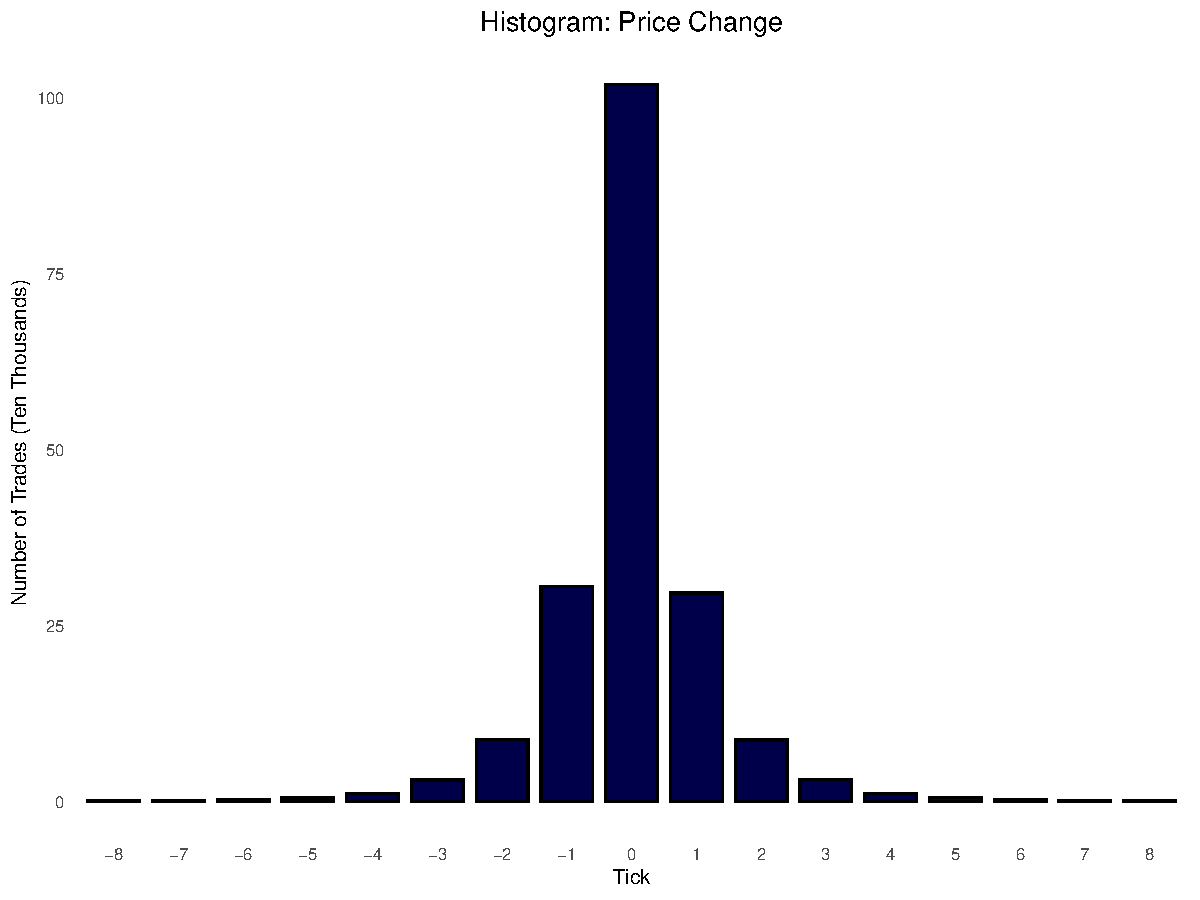
\includegraphics[width=0.8\textwidth]{figures/descriptive stat/price_change_IBM_N_2023.pdf}
    \caption{Histogram of Price Changes: IBM on NYSE, 2023}
    \label{fig:price-change-2023}
\end{figure}







\begin{table}[h]
  \centering
  \setlength{\tabcolsep}{4pt} 
  \resizebox{\textwidth}{!}{%
    \begin{tabular}{@{} r *{14}{r} @{}}
      \toprule
      \textbf{Category}      & 1    & 2       & 3       & 4       & 5       & 6       & 7       & 8       & 9       & 10   
      & 11      & 12      & 13      & 14      \\
      
      \textbf{Price Changes}   & <–6  & [–6,–5) & [–5,–4) & [–4,–3) & [–3,–2) & [–2,–1) & [–1,0)  & [0,1)   & [1,2)   & [2,3)   & [3,4)   & [4,5)   & [5,6)   & \geq6     \\
    
      \textbf{Percentage} & 0.31\% & 0.16\%   & 0.33\%   & 1.83\%   & 2.68\%   & 8.18\%   & 11.08\%  & 62.00\%  & 7.99\%   & 2.68\%   & 1.89\%   & 0.34\%   & 0.17\%   & 0.34\%  \\
      \bottomrule
    \end{tabular}%
  }
  \caption{Frequencies of Partition (Price Changes in Ticks)}
  \label{tab:table-3}
\end{table}

Besides, most of the trade occurs at either higher than or lower than mid-quote prices as similar to the results of \citet{hausman1992} or \citet{kim2014}.

\begin{table}[H]
\centering
\resizebox{0.25\textwidth}{!}{%
\begin{tabular}{ll}
\toprule
\textbf{\% trades at prices} & \\
> Midquote & 40.07\\
= Midquote & 16.65\\
< Midquote & 43.28\\
\textbf{Price change, $Z_k$} & \\
Mean & 0.0000\\
Std. dev. & 0.0134\\
\bottomrule
\end{tabular}}
\caption{Summary statistics: Price Changes}
\label{tab:table-4}
\end{table}



{\noindent\bfseries Trade Direction }

As mentioned in the previous chapter, the trade direction is determined via the procedure proposed by \citet{leeready1991} that incorporates two major steps. Firstly, the trade price is compared with the mid-quote to see if it is greater than mid-quote then it is buyer-initiated trade and vice versa, hereby noted as "mid-quote rule". Secondly, in case the price is equal to the mid-quote then a "tick-test" is applied. The "tick-test" will then compare the current trade with the previous trade's price. If there is again no difference between the two consecutive price then the sign of the last non-zero change will be selected. \citet{hausman1992} adopts only the "mid-quote rule" and thus has the third classification of "indeterminate" trade $IBS = 0$. If we would use the same procedure, our buyer-initiated classfication would simply be the percentage of trade with price > mid-quote (i.e. 40.07\%), and seller-initiated classification would be 43.28\%. Hence, our final results showed in \tabref{tab:table-5} with roughly similar proportion (48.43\% buyer-initiated versus 51.57\% seller-initiated) are reasonable.


\begin{table}[H]
\centering
\resizebox{0.3\textwidth}{!}{%
\begin{tabular}{lr}
\toprule
\textbf{Trade direction, $IBS_k$ }& \\
Buyer-initiated (\%) & 48.43\\
Seller-initiated (\%) & 51.57\\
Mean & -0.0313\\
Std. dev. & 0.9995\\
\bottomrule
\end{tabular}}
\caption{Summary statistics: Trade Direction}
\label{tab:table-5}
\end{table}

{\noindent\bfseries Other Variables }

Last but not least, \tabref{tab:table-6} gives an overview of some other microstructure variables. IBM is traded even more frequently on NYSE with an average of three seconds. This might as well be the effect of high-frequency trading (HFT). The average bid/ask spread is also getting much smaller.













\begin{table}[H]
\centering
\resizebox{0.75\textwidth}{!}{%
\begin{threeparttable}
\begin{tabular}{lrr}
\toprule
Statistic & This Thesis (Panel A) & \citet{hausman1992} \\
\midrule
\textbf{Signed transformed volume}\tnote{a}  & & \\
Mean & -0.1183 & 0.1059 \\
Std. dev. & 4.1303 & 6.1474 \\
\textbf{Time between trades (seconds)} & & \\
Mean & 3.0685 & 27.21 \\
Std. dev. & 10.8139 & 34.13 \\
\textbf{Bid/ask spread} & & \\
Mean & 0.0343 & 1.9470 \\
Std. dev. & 0.0311 & 1.4625 \\
\bottomrule
\end{tabular}
\begin{tablenotes}
    \small
    \item[a] \citet{hausman1992} performs Box-Cox transformation for dollar volume and estimates the \(\lambda\) parameter via maximum likelihood. Their result for IBM is \(\lambda=0\), equivalent to natural log transformation. In this thesis, we simplify by directly taking natural log of dollar volume.
  \end{tablenotes}

\end{threeparttable}}
\caption{Summary statistics: Other Variables}
\label{tab:table-6}
\end{table}




\section{Panel A: Market Microstructure Analysis}

{\noindent\bfseries Maximum Likelihood Estimates  }

\tabref{tab:table-7} presents the maximum likelihood estimates for our ordered probit model. Thirteen partition thresholds for fourteen categories, as well as all parameters for explanatory variables and conditional variance, are statistically significant. While \citet{hausman1992}'s results show negative sign of all lagged price changes $Z_k$ and argue that it might be the sign of price reversal, the same conclusion could not be found for our results.















\begin{table}[H]
\centering
\begin{center}
\resizebox{\textwidth}{!}{%
\begin{threeparttable}
\begin{tabular}{lrlrlr}
\toprule
\multicolumn{1}{c}{\textbf{Parameter}} & \multicolumn{1}{c}{\textbf{Value}} & \multicolumn{1}{c}{\textbf{Thresholds}} & \multicolumn{1}{c}{\textbf{Value}} & \multicolumn{1}{c}{\textbf{Statistics}} & \multicolumn{1}{c}{\textbf{Value}} \\
\midrule
$\beta_1$: $Z_{-1}$ & 0.0319$^{***}$ & $\alpha_1$ & -1.9050$^{***}$ & AIC & 4884659.97 \\
 & (0.0003) & & (0.0036) & & \\
 
$\beta_2$: $Z_{-2}$ & 0.0163$^{***}$ & $\alpha_2$ & -1.7981$^{***}$ & Log Likelihood & -2442306.98 \\
 & (0.0003) & & (0.0031) & & \\
 
$\beta_3$: $Z_{-3}$ & 0.0061$^{***}$ & $\alpha_3$ & -1.6489$^{***}$ & Num. obs. & 1904393 \\
 & (0.0003) & & (0.0026) & & \\
 
$\beta_4$: $IBS_{-1}$ & -0.0433$^{***}$ & $\alpha_4$ & -1.2736$^{***}$ & Iterations & 8 \\
 & (0.0011) & & (0.0017) & & \\
 
$\beta_5$: $IBS_{-2}$ & 0.0149$^{***}$ & $\alpha_5$ & -1.0251$^{***}$ & McFadden's R$^2$ & 0.0743 \\
 & (0.0011) & & (0.0014) & & \\
 
$\beta_6$: $IBS_{-3}$ & 0.0064$^{***}$ & $\alpha_6$ & -0.6611$^{***}$ & & \\
 & (0.0011) & & (0.0009) & & \\
 
$\beta_7$: \(lnV_{-1}\cdot IBS_{-1}\) & 0.0114$^{***}$ & $\alpha_7$ & -0.3961$^{***}$ & & \\
 & (0.0003) & & (0.0007) & & \\
 
$\beta_8$: \(lnV_{-2}\cdot IBS_{-2}\) & 0.0016$^{***}$ & $\alpha_8$ & 0.6121$^{***}$ & & \\
 & (0.0003) & & (0.0009) & & \\
 
$\beta_9$: \(lnV_{-3}\cdot IBS_{-3}\) & 0.0009$^{***}$ &  $\alpha_9$ & 0.9822$^{***}$ & & \\
 & (0.0003) & & (0.0013) & & \\
 
$\gamma$: \(\Delta t/100\) \tnote{a}& 0.1424$^{***}$ & $\alpha_{10}$ & 1.2328$^{***}$ & & \\
 & (0.0002) & & (0.0017) & & \\
 
 & & $\alpha_{11}$ & 1.6137$^{***}$ & & \\
 & & & (0.0025) & & \\
 
 & & $\alpha_{12}$ & 1.7622$^{***}$ & & \\
 & & & (0.0030) & & \\
 
 & & $\alpha_{13}$ & 1.8751$^{***}$ & & \\
 & & & (0.0035) & & \\
\bottomrule
\multicolumn{6}{l}{\scriptsize{$^{***}p<0.001$; $^{**}p<0.01$; $^{*}p<0.05$}}
\end{tabular}

\begin{tablenotes}
    \small
    \item[a] Note: Since the \texttt{oglmx} package \citep{oglmx} only takes the standard deviation argument in the form of \(\sigma=exp(\cdot)\), we take natural log of time between trade variable before estimate the model i.e., \(\sigma=exp(ln(x)) = x\).
  \end{tablenotes}


\end{threeparttable}}
\caption{Ordered Probit Model Estimation}
\label{tab:table-7}
\end{center}
\end{table}



{\noindent\bfseries Impact of Sequence of Trade on the Next Price Change}

As part of a study to explore the impact of trading volume on security price, \citet{easleyohara1987} propose an "information-effects" theory. In this model, the price process will not follow a Markov process i.e. information of the entire sequence of trade is essential to calculate the distribution of the next price, and not only the current price. 

Putting this theory in context of our ordered probit model, \citet{hausman1992} discuss that if the entire sequence of trade would have an impact on the conditional mean of the next price, then one simple case we could test is whether the coefficients ($\beta_1$, $\beta_2$, $\beta_3$) of the lagged price changes different to each other or not. For example, in case the sequence of trade matters, the effect of price change sequence of -1/1/-1 (total change -1 tick) on the conditional mean would be different than 1/-1/-1 (total change also -1 tick). The formulation of the test statistic used by \citet{hausman1992} is similar to a joint Wald test for a linear hypothesis \citep{wooldridge2010}:

\[
\begin{aligned}
H_0 &: \beta_1 = \beta_2 = \beta_3, \\
H_1 &: \text{At least one of } \beta_1, \beta_2, \beta_3 \text{ differs}.
\end{aligned}
\]
    \begin{tabular}{l}
        \textbf{Restriction:}\\
        $Z_{-1} - Z_{-2} = 0$,\\
        $Z_{-2} - Z_{-3} = 0$.\\
        \textbf{Model 1:} restricted model\\
        \textbf{Model 2:} full model, as in \eqref{eq:6}
    \end{tabular}
    
\begin{table}[htbp]
    \centering
    \vspace{0.5em}
    \begin{tabular}{crrl}
        \toprule
        Df & $\chi^2$ & Pr($>$$\chi^2$) \\
        \midrule
         2 & 2823.1 & $<$ 2.2e-16 *** \\ 
         \bottomrule
        \multicolumn{3}{l}{$^{***}p < 0.001$; $^{**}p < 0.01$; $^{*}p < 0.05$}
    \end{tabular}
        \caption{Sequence of Trade: Linear Hypothesis Test}
    \label{tab:table-8}
\end{table}

With this test result, we could reject the null hypothesis at 0.1\% significance level. This finding is consistent with \citet{hausman1992}, and therefore also supports the "information-effects" theory of \citet{easleyohara1987}.



{\noindent\bfseries Impact of Trade Size on the Next Price Change}

In our model, the impact of trade size or volume is measured with variable \(lnV\cdot IBS \). The maximum likelihood estimates in \tabref{tab:table-7} show consistent results with \citet{hausman1992} that the coefficients are significantly positive, and the most recent transaction has the most impact. 

However, the estimated coefficients relate to the impact on the conditional mean of the latent variable $Z_k^*$. \citet{hausman1992} instead attempt to make inference on the impact of trade size on the observed price change $Z_k$. In general, they proceed to calculate the conditional mean for different scenarios following these steps:
\begin{enumerate}
    \item \textbf{Determining specific values for explanatory variables $X_k$}: since our subject-of-interest is the impact of the last trade size, all other variables should be set to identical values while the first-lag of volume varies. The values of these variables are fixed at:
    \begin{itemize}
    \item $V_{-2}$ = $V_{-3}$ = median of dollar volume $\cdot$ $\frac{1}{100}$. 
    (Note that for lagged volumes, although in the original model we have the interaction term between volume and buyer/seller-initiated trade indicator $IBS_k$, here we only include lags of volumes.);
    \item $IBS_{-1}$ = $IBS_{-2}$ = $IBS_{-3}$ = 1 (Assuming the last three transactions are buy-initiated trades);
    \item $\Delta t_k$ = sample mean;
    \end{itemize}
    \item \textbf{Determining sequence-of-trade scenarios}: as the sequence of price change does matter to the conditional mean, we would need to make assumption on the sequences we would like to investigate. Following \citet{hausman1992} there are two cases:
    \begin{itemize}
    \item Increasing price, where $Z_{-1}$ = $Z_{-2}$ = $Z_{-3}$ = +1
    \item Constant price, where $Z_{-1}$ = $Z_{-2}$ = $Z_{-3}$ = 0;
    \end{itemize}
    \item \textbf{Calculating the probabilities}: by substituting the estimated coefficients, with the aforementioned fixed values of $X_k$, based on the conditional distribution \eqref{eq:8};
    \item \textbf{Finally, calculating the expected price};
\end{enumerate}

\tabref{tab:table-9} report the computed conditional means for each specific scenario. The first upper part of the table shows the price impact of trade size in ticks. Since our data in 2023 has much smaller tick size (1 tick = \$0.01) than in 1988 data of \citet{hausman1992} (1 tick = \$0.125), the base price in this thesis is \$500 instead of \$5,000. Following the conditional mean of \$500 are the changes in conditional mean for the next additional dollar volume (e.g. \(\Delta E[Z_k]\) of \$1,000 depicts the change of conditional mean when buying an additional \$500). Moreover, the conditional mean of \$500 is negative, which might be effect by the bid/ask bounce. \citet{hausman1992} argue that while we assume all three previous trades are buys ($IBS_k$ = +1), the next trade could be a sell leading to the negative sign. This effect could be dismissed by calculating the difference in conditional mean for the larger dollar volume than the base \$500, and hence we could still capture the price impact effects of trade size. Our results for both increasing- and constant-price-sequence show the consistent message with their study: a larger trade size would have larger price impact.

Along with the price impact measured in ticks, the price impact in percent of \tabref{tab:table-9} shows the changes as the percentages of the average of the max (\$166.34) and min (\$120.55) trade price. As IBM is a very liquid stock, it is expected that the trade size would have very little impact on price. Moreover, \figref{fig:figure-2} plots the price impact  in percent as a function of the dollar volume i.e., price response function for our IBM stock, conditioning on the increasing-price-sequence as well as the last three trades are buys. A very flat curve again illustrates the high liquid characteristic of IBM \citep{hausman1992}.







\begin{table}[htbp]
\centering

\begin{tabular}{lrr}
\toprule
 & \multicolumn{1}{c}{\$Volume} & \multicolumn{1}{r}{Impact} \\
\midrule
\multicolumn{3}{l}{\textbf{Increasing price sequence (1/1/1)}} \\
\addlinespace[0.5ex]
\multicolumn{3}{l}{\emph{Price impact in ticks}} \\
E$[Z_k]$             &  500   &  $-0.0545$ \\
$\Delta E[Z_k]$      & 1{,}000   &   $0.0943$ \\
$\Delta E[Z_k]$      & 1{,}500   &   $0.1887$ \\
$\Delta E[Z_k]$      & 2{,}000   &   $0.2843$ \\
$\Delta E[Z_k]$      & 2{,}500   &   $0.3818$ \\
$\Delta E[Z_k]$      & 5{,}500   &   $1.0496$ \\
\addlinespace[1ex]
\multicolumn{3}{l}{\emph{Price impact in percent}} \\
E$[Z_k]$             &  500   &  $-0.0004$ \\
$\Delta E[Z_k]$      & 1{,}000   &   $0.0007$ \\
$\Delta E[Z_k]$      & 1{,}500   &   $0.0013$ \\
$\Delta E[Z_k]$      & 2{,}000   &   $0.0020$ \\
$\Delta E[Z_k]$      & 2{,}500   &   $0.0027$ \\
$\Delta E[Z_k]$      & 5{,}500   &   $0.0073$ \\
\midrule
\multicolumn{3}{l}{\textbf{Constant price sequence (0/0/0)}} \\
\addlinespace[0.5ex]
\multicolumn{3}{l}{\emph{Price impact in ticks}} \\
E$[Z_k]$             &  500   &  $-0.1450$ \\
$\Delta E[Z_k]$      & 1{,}000   &   $0.0949$ \\
$\Delta E[Z_k]$      & 1{,}500   &   $0.1891$ \\
$\Delta E[Z_k]$      & 2{,}000   &   $0.2836$ \\
$\Delta E[Z_k]$      & 2{,}500   &   $0.3793$ \\
$\Delta E[Z_k]$      & 5{,}500   &   $1.0217$ \\
\addlinespace[1ex]
\multicolumn{3}{l}{\emph{Price impact in percent}} \\
E$[Z_k]$             &  500   &  $-0.0010$ \\
$\Delta E[Z_k]$      & 1{,}000   &   $0.0007$ \\
$\Delta E[Z_k]$      & 1{,}500   &   $0.0013$ \\
$\Delta E[Z_k]$      & 2{,}000   &   $0.0020$ \\
$\Delta E[Z_k]$      & 2{,}500   &   $0.0026$ \\
$\Delta E[Z_k]$      & 5{,}500   &   $0.0071$ \\
\bottomrule
\end{tabular}

\caption{Impact of Trade Size.}
\label{tab:table-9}
\end{table}




\begin{figure}[H]
    \centering
    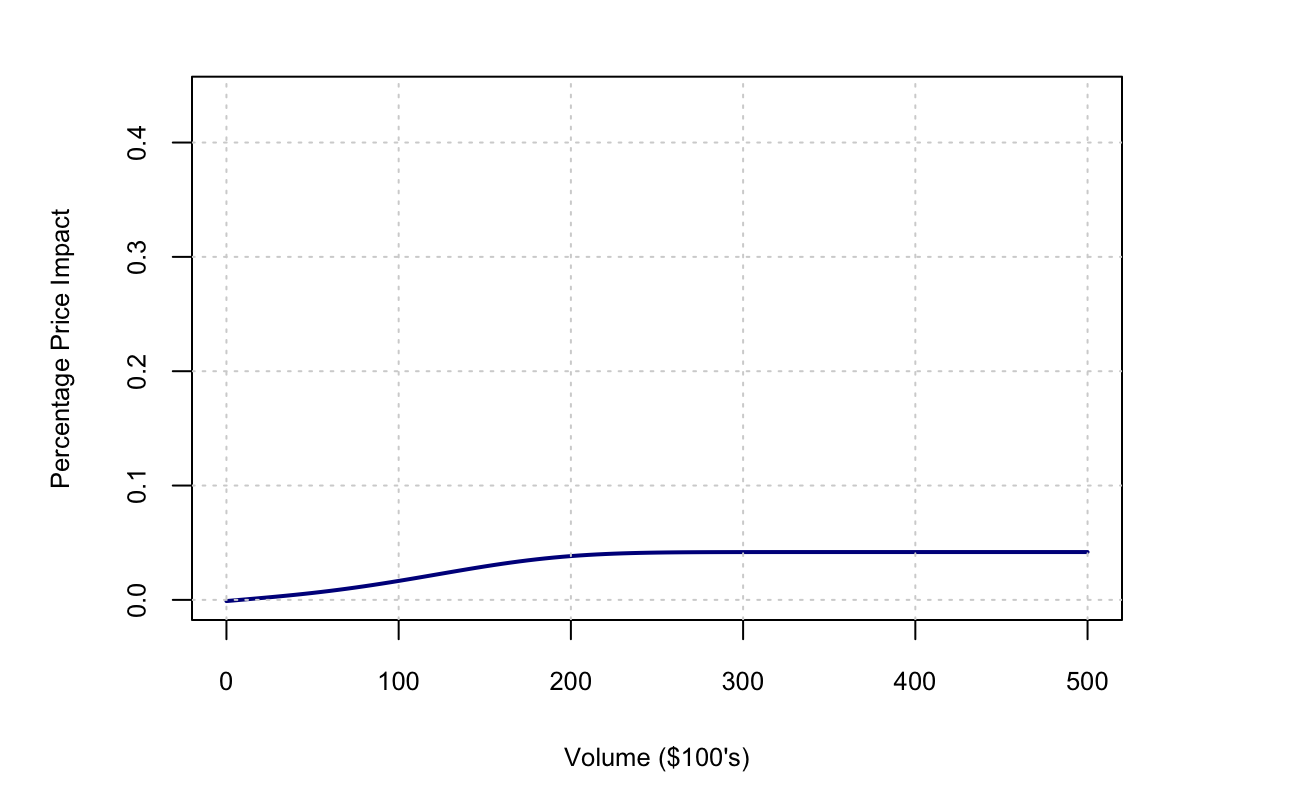
\includegraphics[width=1.1\textwidth]{figures/main_results/price_response.png}
    \caption{Price Response Function for IBM on NYSE, 2023.}
    \label{fig:figure-2}
\end{figure}


\clearpage



\section{Panel B: Forecasting Analysis}

{\noindent\bfseries In-sample }

Our in-sample period from January 2023 to October 2023 is first estimated with the ordered probit model as in the previous section. \tabref{tab:table-10} presents the maximum likelihood estimation results. Similar to the full sample estimation, our in-sample's coefficients are all statistically significant. The pseudo $R^2$ i.e., McFadden's $R^2$ is also low as expected, nevertheless when we would like to extend the model (e.g. add more explanatory variables) we could use this as an evaluation metric.






\begin{table}[H]
\centering
\begin{center}
\resizebox{\textwidth}{!}{%
\begin{threeparttable}
\begin{tabular}{lrlrlr}
\toprule
\multicolumn{1}{c}{\textbf{Parameter}} & \multicolumn{1}{c}{\textbf{Value}} & \multicolumn{1}{c}{\textbf{Thresholds}} & \multicolumn{1}{c}{\textbf{Value}} & \multicolumn{1}{c}{\textbf{Statistics}} & \multicolumn{1}{c}{\textbf{Value}} \\
\midrule
$\beta_1$: $Z_{-1}$ & 0.0303$^{***}$ & $\alpha_1$ & -1.8903$^{***}$ & AIC & 4226828.7780 \\
 & (0.0004) & & (0.0038) & & \\
 
$\beta_2$: $Z_{-2}$ & 0.0157$^{***}$ & $\alpha_2$ & -1.7849$^{***}$ & Log Likelihood & -2113391.3890 \\
 & (0.0004) & & (0.0033) & & \\
 
$\beta_3$: $Z_{-3}$ & 0.0059$^{***}$ & $\alpha_3$ & -1.6331$^{***}$ & Num. obs. & 1640858 \\
 & (0.0004) & & (0.0027) & & \\
 
$\beta_4$: $IBS_{-1}$ & -0.0403$^{***}$ & $\alpha_4$ & -1.2617$^{***}$ & Iterations & 8 \\
 & (0.0012) & & (0.0018) & & \\
 
$\beta_5$: $IBS_{-2}$ & 0.0136$^{***}$ & $\alpha_5$ & -1.0195$^{***}$ & McFadden's R$^2$ & 0.0748 \\
 & (0.0012) & & (0.0014) & & \\
 
$\beta_6$: $IBS_{-3}$ & 0.0056$^{***}$ & $\alpha_6$ & -0.6513$^{***}$ & & \\
 & (0.0012) & & (0.0010) & & \\
 
$\beta_7$: \(lnV_{-1}\cdot IBS_{-1}\) & 0.0110$^{***}$ & $\alpha_7$ & -0.3930$^{***}$ & & \\
 & (0.0003) & & (0.0007) & & \\
 
$\beta_8$: \(lnV_{-2}\cdot IBS_{-2}\) & 0.0017$^{***}$ & $\alpha_8$ & 0.6026$^{***}$ & & \\
 & (0.0003) & & (0.0010) & & \\
 
$\beta_9$: \(lnV_{-3}\cdot IBS_{-3}\) & 0.0010$^{***}$ &  $\alpha_9$ & 0.9764$^{***}$ & & \\
 & (0.0003) & & (0.0014) & & \\
 
$\gamma$: \(\Delta t/100\) & 0.1432$^{***}$ & $\alpha_{10}$ & 1.2210$^{***}$ & & \\
 & (0.0002) & & (0.0018) & & \\
 
 & & $\alpha_{11}$ & 1.5978$^{***}$ & & \\
 & & & (0.0027) & & \\
 
 & & $\alpha_{12}$ & 1.7484$^{***}$ & & \\
 & & & (0.0032) & & \\
 
 & & $\alpha_{13}$ & 1.8597$^{***}$ & & \\
 & & & (0.0037) & & \\
\bottomrule
\multicolumn{6}{l}{\scriptsize{$^{***}p<0.001$; $^{**}p<0.01$; $^{*}p<0.05$}}
\end{tabular}
\end{threeparttable}}
\caption{In-sample Estimation (January 3 - October 31, 2023).}
\label{tab:table-10}
\end{center}
\end{table}


\begin{figure}[H]
    \centering
    \resizebox{0.85\textwidth}{!}{%
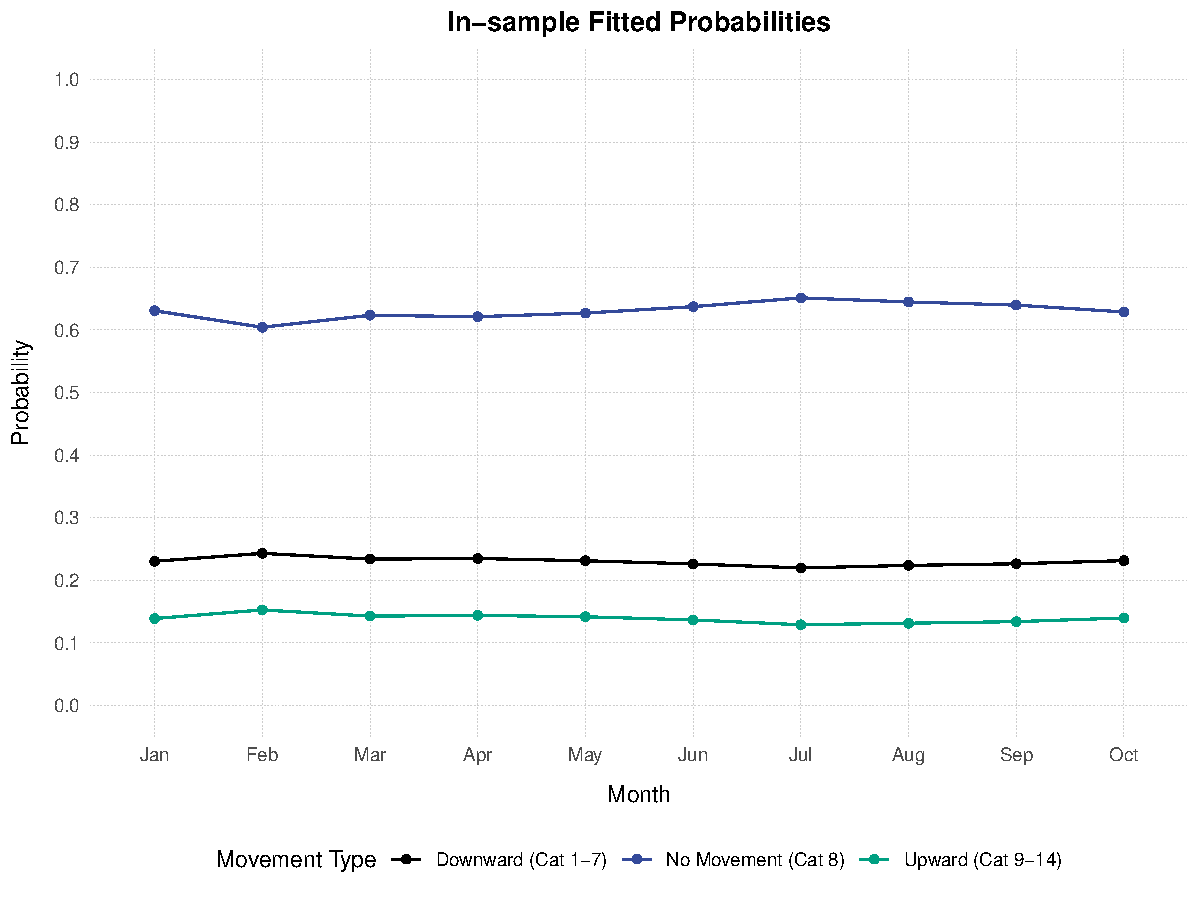
\includegraphics{figures/main_results/monthly_probabilities_in_sample.pdf}}
    \caption{Aggregated Monthly Fitted Probability for In-sample Period (January - October 2023).}
    \label{fig:figure-3}
\end{figure}

To have an easier interpretation regarding the transaction price movement, we could cluster our 14 categories into three major movement: downward movement (category 1 to 7), no change (category 8), and upward movement (category 9 to 14). (The definition of each category could be reviewed in \tabref{tab:table-3}.) \figref{fig:figure-3} illustrates the average monthly fitted probability for the in-sample observations. The sum of fitted probability of falling into each category for each observation equals to 1. Accordingly, the \textit{no movement} category has the highest fitted probability.














{\noindent\bfseries Out-of-sample }
